\section{Discussion}
\label{chap:Discussion}

\subsection{Part A}
\label{chap:PartA}

\subsubsection{Ordinary Least Squares, Ridge regression and Stochastic Gradient Descent on terrain's heights GeoTIF image-data}
\label{chap:Ordinary Least Squares, Ridge regression and Stochastic Gradient Descent on terrain's heights GeoTIF image-data}

\qquad \, We start part A of this project with a re-capitulation of \href{https://github.com/fabiorodp/UiO-FYS-STK4155/blob/master/Project1}{[Project 1]}, part F and G, where a GeoTIF terrain image, containing the heights of a region near Stavanger/Norway, was extracted and examined on Ordinary Least Squares (OLS) and Ridge regression models. On that occasion, we generated two sets of explanatory variables ($\boldsymbol{x1}$, $\boldsymbol{x2}$), with values between 0 and 1, and utilized them on the design matrix ($\boldsymbol{X}$) function that performed a polynomial transformation with a degree equals 10 for OLS and 11 for Ridge. The response variable set ($\boldsymbol{z}$) had space (number of samples or size of the sliced image) of 15 (15x15 pixels). Lastly, the testing MSE (mean squared error) scores obtained were 1.11 and 1.44 for OLS and Ridge, respectively.\\

Now, we perform a Stochastic Gradient Descent (SGD) utilizing the same generated data as above. It is essential to say that we do not scale the data-sets because of possible crashes during the gradient computations. The \href{https://github.com/fabiorodp/UiO-FYS-STK4155/blob/master/Project2/package/gradient_descent.py}{[gradient\_descent.py]} under the \href{https://github.com/fabiorodp/UiO-FYS-STK4155/tree/master/Project2/package}{[Project2/package/]} directory has the algorithms for GDM and Mini-SGDM.\\

Our first experiment for SGD is a Grid-Search, also incorporated at the \href{https://github.com/fabiorodp/UiO-FYS-STK4155/tree/master/Project2/package}{[Project2/package/]} directory with the file name \href{https://github.com/fabiorodp/UiO-FYS-STK4155/blob/master/Project2/package/grid_search.py}{[grid\_search.py]}. We run the Grid-Search class to find the best constant learning rate ($\eta$ = [0.02, 0.01, 0.005, 0.001, 0.0005]) as function of the number of interactions (epochs=[100, 500, 1000, 5000, 10000]). The model applied to the Grid-Search is the MiniSGDM class, which is an SGD when the number of batches is equal to 1, gamma=0, lambda=0, and decay=0.\\

The results are as follows:\\

\begin{figure}[H]
\label{fig:figA1}
\centering
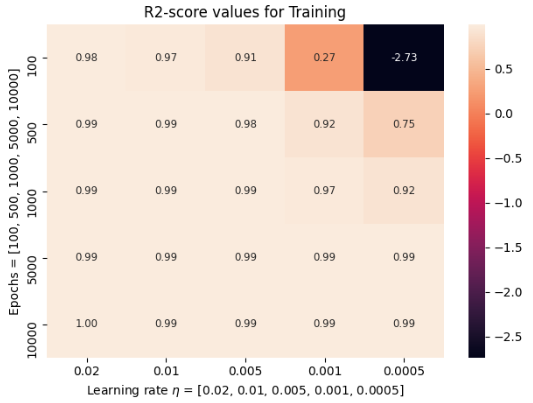
\includegraphics[width=7cm]{heatmapA1}
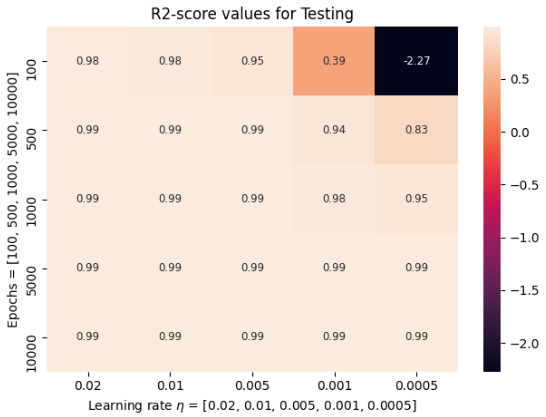
\includegraphics[width=7cm]{heatmapA2}
\caption{Heat-map containing the R2-score training and testing results of a Grid-Search with Learning rates = [0.02, 0.01, 0.005, 0.0001, 0.0005] and epochs = [100, 500, 1000, 5000, 10000].}
\end{figure}\\

As one can see, the design matrix ($\boldsymbol{X}$) with degree equals to 10 explains the response variable ($\boldsymbol{z}$) at a rate of 99 percent, according to the r2-scores in \hyperref[fig:figA1]{[Fig.1]}. In other words, these results suggest that the input polynomials translate almost entirely the output heights of the terrain region studied.\\

\begin{figure}[H]
\label{fig:figA2}
\centering
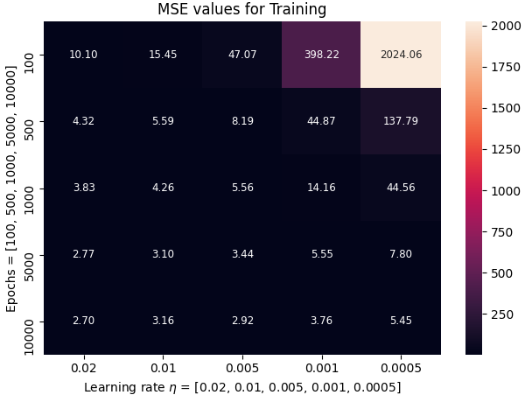
\includegraphics[width=7cm]{heatmapA3}
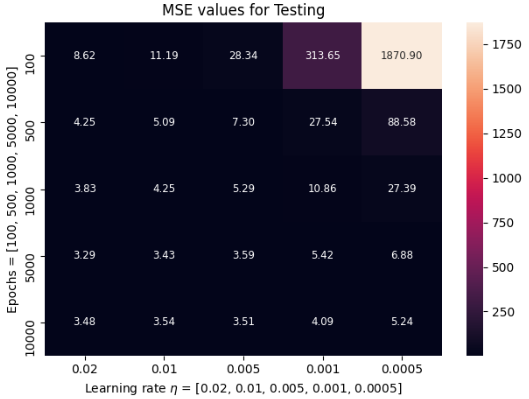
\includegraphics[width=7cm]{heatmapA4}
\caption{Heat-map containing the MSE training and testing results of a Grid-Search with Learning rates = [0.02, 0.01, 0.005, 0.0001, 0.0005] and epochs = [100, 500, 1000, 5000, 10000]. }
\end{figure}\\

The results from training and testing heat-maps \hyperref[fig:fidA2]{[Fig.2]} shows that the best testing MSE scores are between 3.3 and 3.4, for learning rates 0.02 and 0.01, respectively, and epochs 5000. Notice that as the number of epochs increases, the MSE scores decreases until a certain point and then increases again. We then choose the number of epochs equals 5000 as the parameter's benchmarks on futures experiments.\\

\subsubsection{Tuning computation's cost (mini-batches)}
\label{chap:Tuning computation's cost (mini-batches)}

\qquad \, The SGD method with a unique mini-batch is costly for computations while fitting the model. The algorithm stochastically chooses a single vector of features from the sample space, calculates the gradient, and updates the weights. This process is repeated for as many samples in the design matrix ($\boldsymbol{X}$) for every epoch. It turns out that the number of computations sky rocks and the entire fitting takes a long time to complete, as shown on the heat-map below:

\begin{figure}[H]
\label{fig:figA3}
\centering
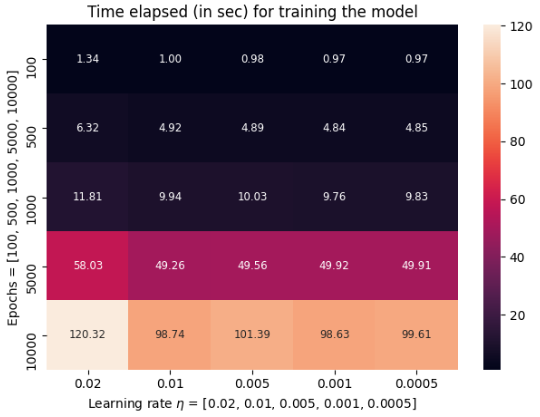
\includegraphics[width=8cm]{heatmapA5}
\caption{Heat-map containing the fitting time (in seconds) of the previous Grid-Search on \hyperref[fig:figA1]{[Fig.1]} and \hyperref[fig:figA2]{[Fig.2]}.}
\end{figure}\\

It is evident that as the number of epochs is high, the computations' costs are higher. For example, our model's fitting time takes approx. 2 seconds to run when the epoch number is 100. On the other hand, when the epoch is 10000, the fitting time is 2 minutes and 40 seconds.\\

To avoid the cost of this expensive computation, we introduce the mini-batches technique. Instead of stochastically choosing only one vector of features from the training sample, the algorithm chooses feature vectors blocks.\\

Therefore, we perform a Grid-Search for the parameters etas=[0.01, 0.005, 0.001, 0.0005] and batch\_sizes=[1, 5, 10, 15, 20], using our bench-marked epoch value equal 5.000, and analyse the testing MSE performance and fitting's time on the heat-maps below:\\

\begin{figure}[H]
\label{fig:figA4}
\centering
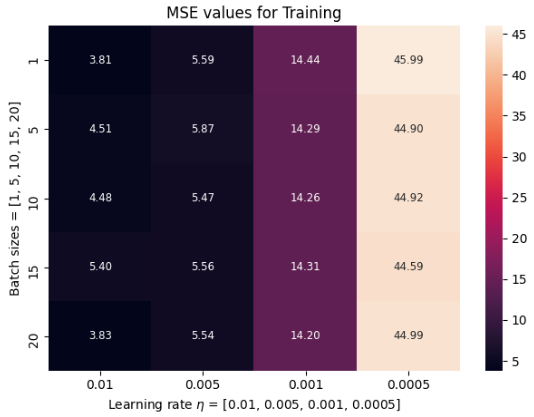
\includegraphics[width=7cm]{heatmapA6}
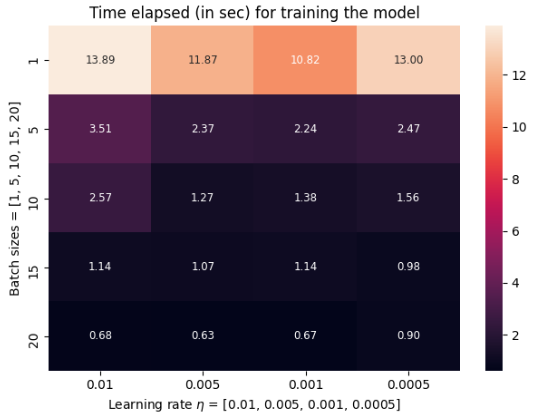
\includegraphics[width=7cm]{heatmapA7}
\caption{Left heat-map shows the testing MSE scores for each search. Right heat-map shows the fitting's time for each search.}
\end{figure}\\

For a single vector of features (batch\_size=1), the elapsed fitting's times are above 60 seconds. Under blocks of feature vectors (mini-batches), the elapsed fitting times have a tremendous reduction, of more than 90 percent, without losing the accuracy. For example, the case with learning rate=0.005 and batch-size=1 got MSE equals 3.50, and fitting's time equals 63 seconds, however for the same learning rate=0.005, but batch\_size=10, the fitting's time was more than ten times faster, and with even better testing MSE score equals 3.49.\\

Hence, we define our bench-marked parameters epochs=5.000, batch\_size=10, for futures examinations. We will try to beat the best testing MSE of 3.41 obtained in this section by introducing learning rate decay, momentum gamma, and 'l2' regularization.\\

\subsubsection{Learning rate decay and tuning decay}
\label{chap:Learning rate decay and tuning decay}

\qquad \, There are many ways to optimize the learning rate to find more accurate predictions. As studied in \hyperref[chap:Learning Rate]{[Learning rate theory]}, the learning rate ($\eta$) is a hyper-parameter that manages the model's change in response to the MSE each time the model's coefficients (weights) are updated.\\

Now, we apply a technique that reduces the learning rate value according to the number of epochs. To do that, we introduce a constant parameter called decay.\\

Thus, we run a Grid-search with the parameters etas=[0.01, 0.005, 0.001, 0.0005] and decays=[10**-1, 10**-2, 10**-3, 10**-4, 10**-5, 10**-6, 10**-7], using our bench-marked epoch=5.000 and batch-size=10, to find the best testing MSE score for an eta as a function of the decay value:\\

\begin{figure}[H]
\label{fig:figA5}
\centering
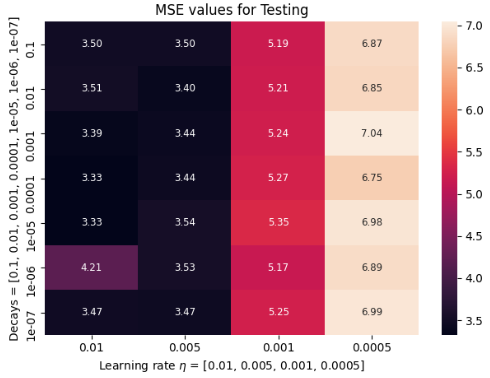
\includegraphics[width=8cm]{heatmapA8}
\caption{Heat-map showing the testing MSE scores for learning rates as function of decays.}
\end{figure}\\

Comparing the testing MSE scores from \hyperref[fig:figA4]{[Fig.4]} and \hyperref[fig:figA5]{[Fig.5]}, there is an significant improvement when a eta-decay parameter is applied. Before, \hyperref[fig:figA4]{[Fig.4]} shows that, for batch-size=10 with decay=0, the testing MSE scores are [3.85, 3.49, 5.25, 6.97] for learning rates [0.01, 0.005, 0.001, 0.0005]. Now, for the same batch-size=10 and different decay=0.0001, the testing MSE scores are [3.33, 3.44, 5.27, 6.75] for the same learning-rates.\\

Hence, we include decay=0.0001 and eta0=0.01 to our bench-marked parameters epochs=5.000, batch\_size=10. We will try to beat the testing MSE of 3.33 obtained in this section by introducing momentum gamma and 'l2' regularization in the following sub-sections.\\


\subsubsection{SGD with momentum and tuning gamma}
\label{chap:SGD with momentum and tuning gamma}

\qquad \, This subsection will try to overcome the testing MSE of 3.33 by applying another type of Stochastic Gradient Descent, so-called SGD with momentum. A new parameter gamma is introduced, as explained in the theory section in \hyperref[chap:Stochastic Gradient Decedent]{[here]}. We use different values of gamma=[0.2, 0.3, 0.35, 0.4, 0.45, 0.5, 0.6, 0.7] and run the model \href{https://github.com/fabiorodp/UiO-FYS-STK4155/blob/master/Project2/package/gradient_descent.py}{[MiniSGDM]} with the bench-marked parameters obtained from the previous subsections, decay=0.0001, eta0=0.01, epochs=5.000 and batch\_size=10.\\

\begin{figure}[H]
\label{fig:figA6}
\centering
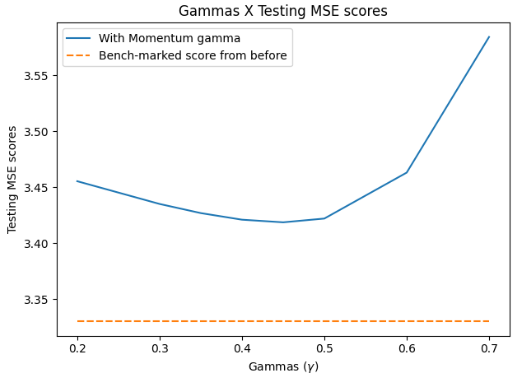
\includegraphics[width=8cm]{plotA1}
\caption{Line-plot containing the MSE values as function of gammas.}
\end{figure}\\

As shown, the Mini-batch Stochastic Gradient Descent with momentum got closer to our bench-mark score of 3.33 but did not overcome.\\

\subsubsection{'L2' regularization and tuning lambda}
\label{chap:'L2' regularization and tuning lambda}

\qquad \, This subsection will try to overcome the testing MSE of 3.33 by applying the l2 regularization (Ridge). A new parameter lambda is introduced, as explained in the theory section in \hyperref[chap:Stochastic Gradient Decedent]{[here]}. We use different values of lambda=[10**-6, 10**-5, 10**-4, 10**-3] and run the model \href{https://github.com/fabiorodp/UiO-FYS-STK4155/blob/master/Project2/package/gradient_descent.py}{[MiniSGDM]} with the bench-marked parameters obtained from the previous subsections, gamma=0, decay=0.0001, eta0=0.01, epochs=5.000 and batch\_size=10.\\

\begin{figure}[H]
\label{fig:figA7}
\centering
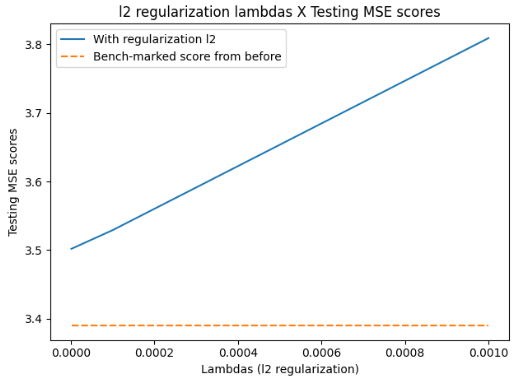
\includegraphics[width=8cm]{plotA2}
\caption{Line-plot containing the MSE values as function of lambdas.}
\end{figure}\\

As exhibited, the 'l2' regularization did not make any improvement overcoming our bench-mark of 3.33.\\

\subsection{Part B and C}
\label{chap:Part B and C}

\subsubsection{Terrain GeoTIF image/data on Deep Neural Networks}
\label{chap:Terrain GeoTIF image/data on Deep Neural Networks}

